\documentclass{beamer}
\usepackage{tikz,amsmath,hyperref,graphicx,stackrel,animate}
\usetikzlibrary{positioning,shadows,arrows,shapes,calc}
\newcommand{\argmax}{\operatornamewithlimits{argmax}}
\newcommand{\argmin}{\operatornamewithlimits{argmin}}
\mode<presentation>{\usetheme{Frankfurt}}
\AtBeginSection[]
{
  \begin{frame}<beamer>
    \frametitle{Outline}
    \tableofcontents[currentsection,currentsubsection]
  \end{frame}
}
\title{Lecture 3: Spectrum}
\author{Mark Hasegawa-Johnson}
\date{ECE 401: Signal and Image Analysis, Fall 2022}  
\begin{document}

% Title
\begin{frame}
  \maketitle
\end{frame}

% Title
\begin{frame}
  \tableofcontents
\end{frame}

%%%%%%%%%%%%%%%%%%%%%%%%%%%%%%%%%%%%%%%%%%%%
\section[Beating]{Beat Tones}
\setcounter{subsection}{1}

\begin{frame}
  \frametitle{Beat tones}

  When two pure tones at similar frequencies are added together, you hear the  two tones
  ``beating'' against each other.
  \vspace*{1cm}
  \centerline{\fbox{\href{https://en.wikipedia.org/wiki/Beat_(acoustics)}{Beat tones demo}}}
\end{frame}

\begin{frame}
  \frametitle{Beat tones and Trigonometric identities}

  Beat tones can be explained using this trigonometric identity:
  \[
  \cos(a)\cos(b)=\frac{1}{2}\cos(a+b)+\frac{1}{2}\cos(a-b)
  \]
  Let's do the following variable substitution:
  \begin{align*}
    a+b &= 2\pi f_1 t\\
    a-b &= 2\pi f_2 t\\
    a &= 2\pi f_{ave}t\\
    b &= 2\pi f_{beat}t
  \end{align*}
  where $f_{ave}=\frac{f_1+f_2}{2}$, and $f_{beat}=\frac{f_1-f_2}{2}$.
\end{frame}

\begin{frame}
  \frametitle{Beat tones and Trigonometric identities}

  Re-writing the trigonometric identity, we get:
  \[
  \frac{1}{2}\cos(2\pi f_1t)+\frac{1}{2}\cos(2\pi f_2 t) = \cos(2\pi f_{beat}t)\cos(2\pi f_{ave}t)
  \]
  So when we play two tones together, $f_1=110$Hz and $f_2=104$Hz, it
  sounds like we're playing a single tone at $f_{ave}=107$Hz,
  multiplied by a beat frequency $f_{beat}=3$ (double beats)/second.
\end{frame}

\begin{frame}
  \frametitle{Beat tones\\\begin{tiny}by Adjwilley, CC-SA 3.0,
    \url{https://commons.wikimedia.org/wiki/File:WaveInterference.gif}\end{tiny}}
  \centerline{\animategraphics[loop,controls,height=2.5in]{20}{exp/WaveInterference-}{0}{125}}
\end{frame}

\begin{frame}
  \frametitle{More complex beat tones}

  What happens if we add together, say, three tones?
  \[
  \cos(2\pi 107t) + \cos(2\pi 110t)+\cos(2\pi 104t)=\mbox{???}
  \]
  For this, and other more complicated operations, it
  is much, much easier to work with complex exponentials, instead of cosines.
\end{frame}
  

\begin{frame}
  \frametitle{More complex beat tones}

  What happens if we add together, say, three tones?
  \[
  x(t) = \cos(2\pi 107t) + \cos(2\pi 110t)+\cos(2\pi 104t)=\mbox{???}
  \]
  This is like a phasor example, except that all of the tones are at
  different frequencies.
  \begin{align*}
    x(t) &= \Re\left\{e^{j2\pi 107t}+e^{j2\pi 110t}+e^{j2\pi 104t}\right\}\\
    &= \Re\left\{\left(1+e^{j2\pi 3t}+e^{-j2\pi 3t}\right)e^{j2\pi 107t}\right\}
  \end{align*}
  So we just have to do this phasor addition:
  \[
  1+e^{j2\pi 3t}+e^{-j2\pi 3t} = 1 + 2\cos\left(2\pi 3t\right)
  \]
\end{frame}

\begin{frame}
  \frametitle{Triple-beat example}

  \centerline{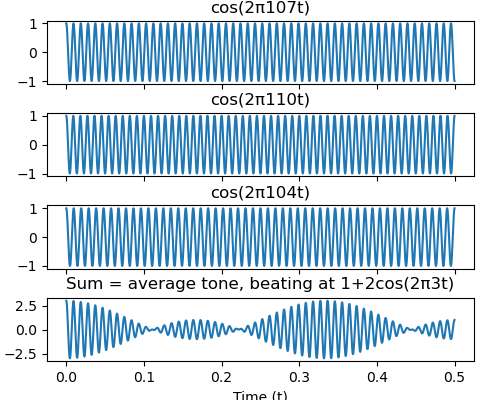
\includegraphics[height=3in]{exp/triplebeat.png}}
\end{frame}

%%%%%%%%%%%%%%%%%%%%%%%%%%%%%%%%%%%%%%%%%%%%
\section[Spectrum]{Spectrum}
\setcounter{subsection}{1}

\begin{frame}
  \frametitle{Phasor representation of a general sum of sinusoids}

  In general, if $x(t)$ is a sum of sines and cosines,
  \[
  x(t) = A_0 + \sum_{k=1}^N A_k\cos\left(2\pi f_kt+\theta_k\right)
  \]
  Then it has a phasor notation
  \[
  x(t) = A_0+\sum_{k=1}^N\Re\left\{A_ke^{j\theta_k}e^{j2\pi f_kt}\right\}
  \]
\end{frame}

\begin{frame}
  \frametitle{Two-sided spectrum}

  The $\Re\left\{z\right\}$ operator is annoying.  In order to get rid
  of it, let's take advantage of Euler's formula
  $\Re\left\{z\right\}=\frac{1}{2}(z+z^*)$ to write:
  \begin{align*}
    x(t) &= A_0+ \sum_{k=1}^N A_k\cos\left(2\pi f_kt+\theta_k\right)\\
    &= \sum_{k=-N}^N a_k e^{j2\pi f_k t}    
  \end{align*}
  In order to do that, we need to define $a_k$ like this:
  \[
  a_k = \begin{cases}
    A_0 & k=0\\
    \frac{1}{2}A_ke^{j\theta_k} & k>0\\
    \frac{1}{2}A_{-k}e^{-j\theta_{-k}} & k < 0
  \end{cases}
  \]  
\end{frame}

\begin{frame}
  \frametitle{Two-sided spectrum}

  The {\bf spectrum} of $x(t)$ is the set of frequencies, and their
  associated phasors,
  \[
  \mbox{Spectrum}\left( x(t) \right) =
  \left\{ (f_{-N},a_{-N}), \ldots, (f_0,a_0), \ldots, (f_N,a_N) \right\}
  \]
  such that
  \[
  x(t) = \sum_{k=-N}^N a_ke^{j2\pi f_kt}
  \]
\end{frame}

%%%%%%%%%%%%%%%%%%%%%%%%%%%%%%%%%%%%%%%%%%%%
\section[Periodic]{Periodic Signals}
\setcounter{subsection}{1}

\begin{frame}
  \frametitle{Fourier's theorem}

  One reason the spectrum is useful is that {\bf\em any} periodic
  signal can be written as a sum of cosines.  Fourier's theorem says that
  any $x(t)$ that is periodic, i.e.,
  \[
  x(t+T_0) = x(t)
  \]
  can be written as
  \[
  x(t) = \sum_{k=-\infty}^\infty X_k e^{j2\pi k F_0 t}
  \]
  which is a special case of the spectrum for periodic signals:
  $f_k=kF_0$, and $a_k=X_k$, and
  \[
  F_0 = \frac{1}{T_0}
  \]
\end{frame}

\begin{frame}
  \frametitle{Analysis and Synthesis}

  \begin{itemize}
  \item {\bf Fourier Analysis} is the process of finding the spectrum,
    $X_k$, given the signal $x(t)$.  I'll tell you how to do that next lecture.
  \item {\bf Fourier Synthesis} is the process of generating the
    signal, $x(t)$, given its spectrum.  I'll spend the rest of
    today's lecture showing examples and properties of synthesis.
  \end{itemize}
\end{frame}

\begin{frame}
  \frametitle{Example: Square wave}

  \centerline{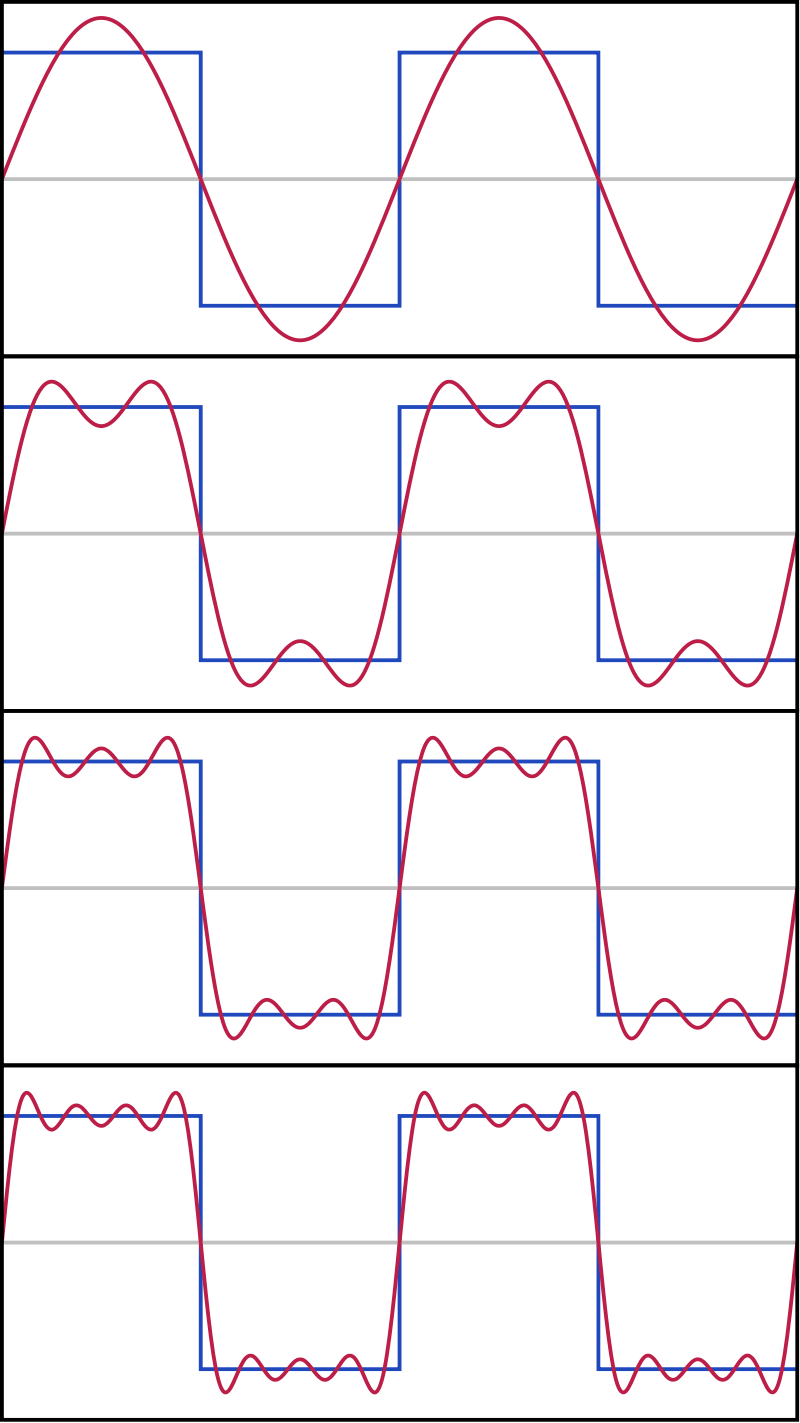
\includegraphics[height=2.5in]{squarewave.png}}
  \begin{tiny}
    Jim.belk, Public domain image 2009,
    \url{https://commons.wikimedia.org/wiki/File:Fourier_Series.svg}
  \end{tiny}
\end{frame}

\begin{frame}
  \frametitle{Example \#1: Square wave}

  \centerline{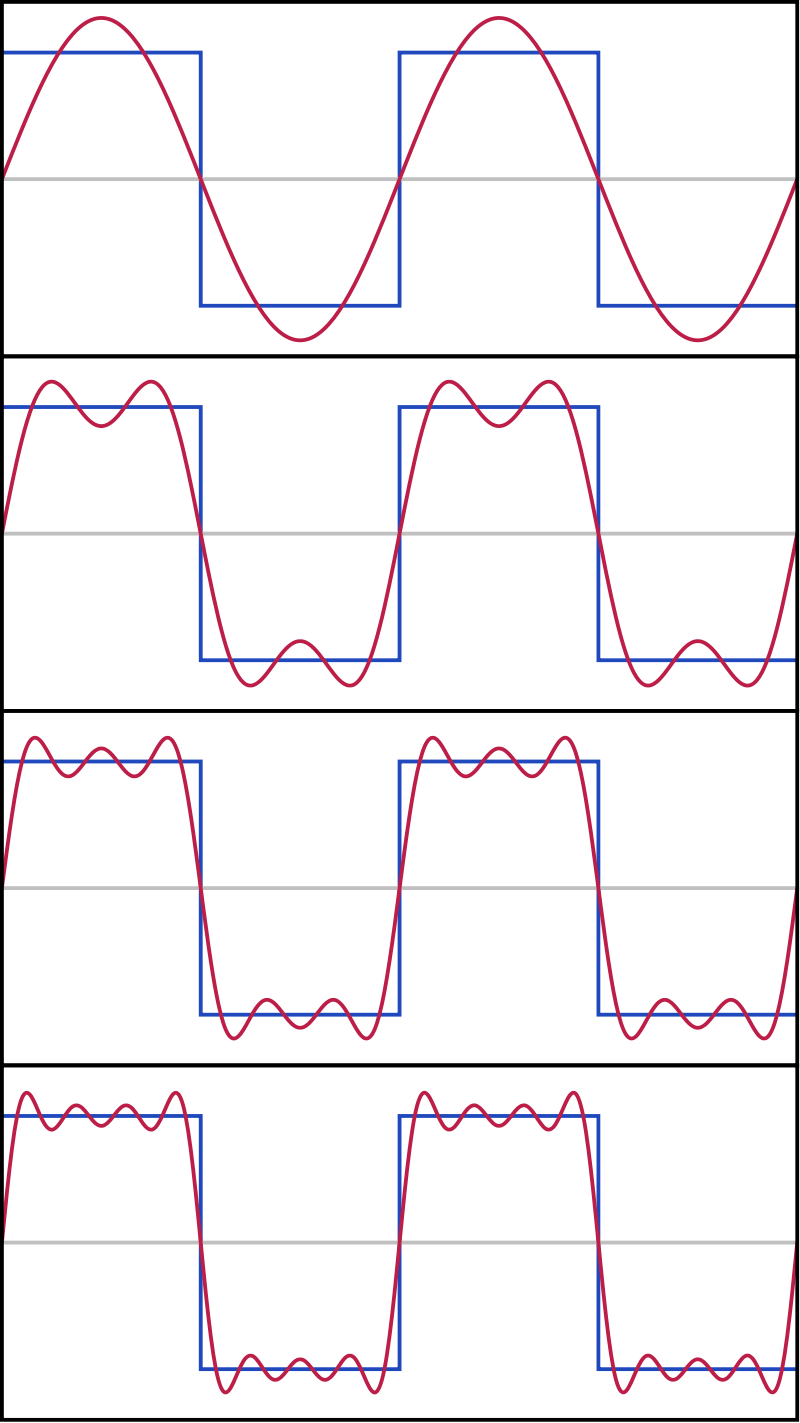
\includegraphics[height=2.5in]{squarewave.png}}
  \begin{tiny}
    Jim.belk, Public domain image 2009,
    \url{https://commons.wikimedia.org/wiki/File:Fourier_Series.svg}
  \end{tiny}
\end{frame}

\begin{frame}
  \frametitle{Example \#1: Square wave\\\begin{tiny}
    \url{https://upload.wikimedia.org/wikipedia/commons/b/bd/Fourier_series_square_wave_circles_animation.svg}\end{tiny}}
    
  \centerline{\animategraphics[loop,controls,height=2.5in]{20}{exp/squarewave_animation-}{0}{59}}
\end{frame}

\begin{frame}
  \frametitle{Example \#2: Sawtooth wave\\\begin{tiny}By Lucas Vieira, public domain 2009,
    \url{https://commons.wikimedia.org/wiki/File:Periodic_identity_function.gif}\end{tiny}}
    
  \centerline{\animategraphics[loop,controls,height=1in]{2}{exp/sawtooth_anim1-}{0}{4}}
\end{frame}

\begin{frame}
  \frametitle{Example \#2: Sawtooth wave\\\begin{tiny}
    \url{https://upload.wikimedia.org/wikipedia/commons/1/1e/Fourier_series_sawtooth_wave_circles_animation.svg}\end{tiny}}
    
  \centerline{\animategraphics[loop,controls,height=2.5in]{20}{exp/sawtooth_anim2-}{0}{59}}
\end{frame}

\begin{frame}
  \frametitle{Example: A weird arbitrary signal\\\begin{tiny}By Scallop7, CC-SA 4.0 2007,
    \url{https://commons.wikimedia.org/wiki/File:Example_of_Fourier_Convergence.gif}\end{tiny}}
    
  \centerline{\animategraphics[loop,controls,height=2.5in]{20}{exp/Fourier_Convergence-}{0}{99}}
\end{frame}

\begin{frame}
  \frametitle{Example: Violin}

  \centerline{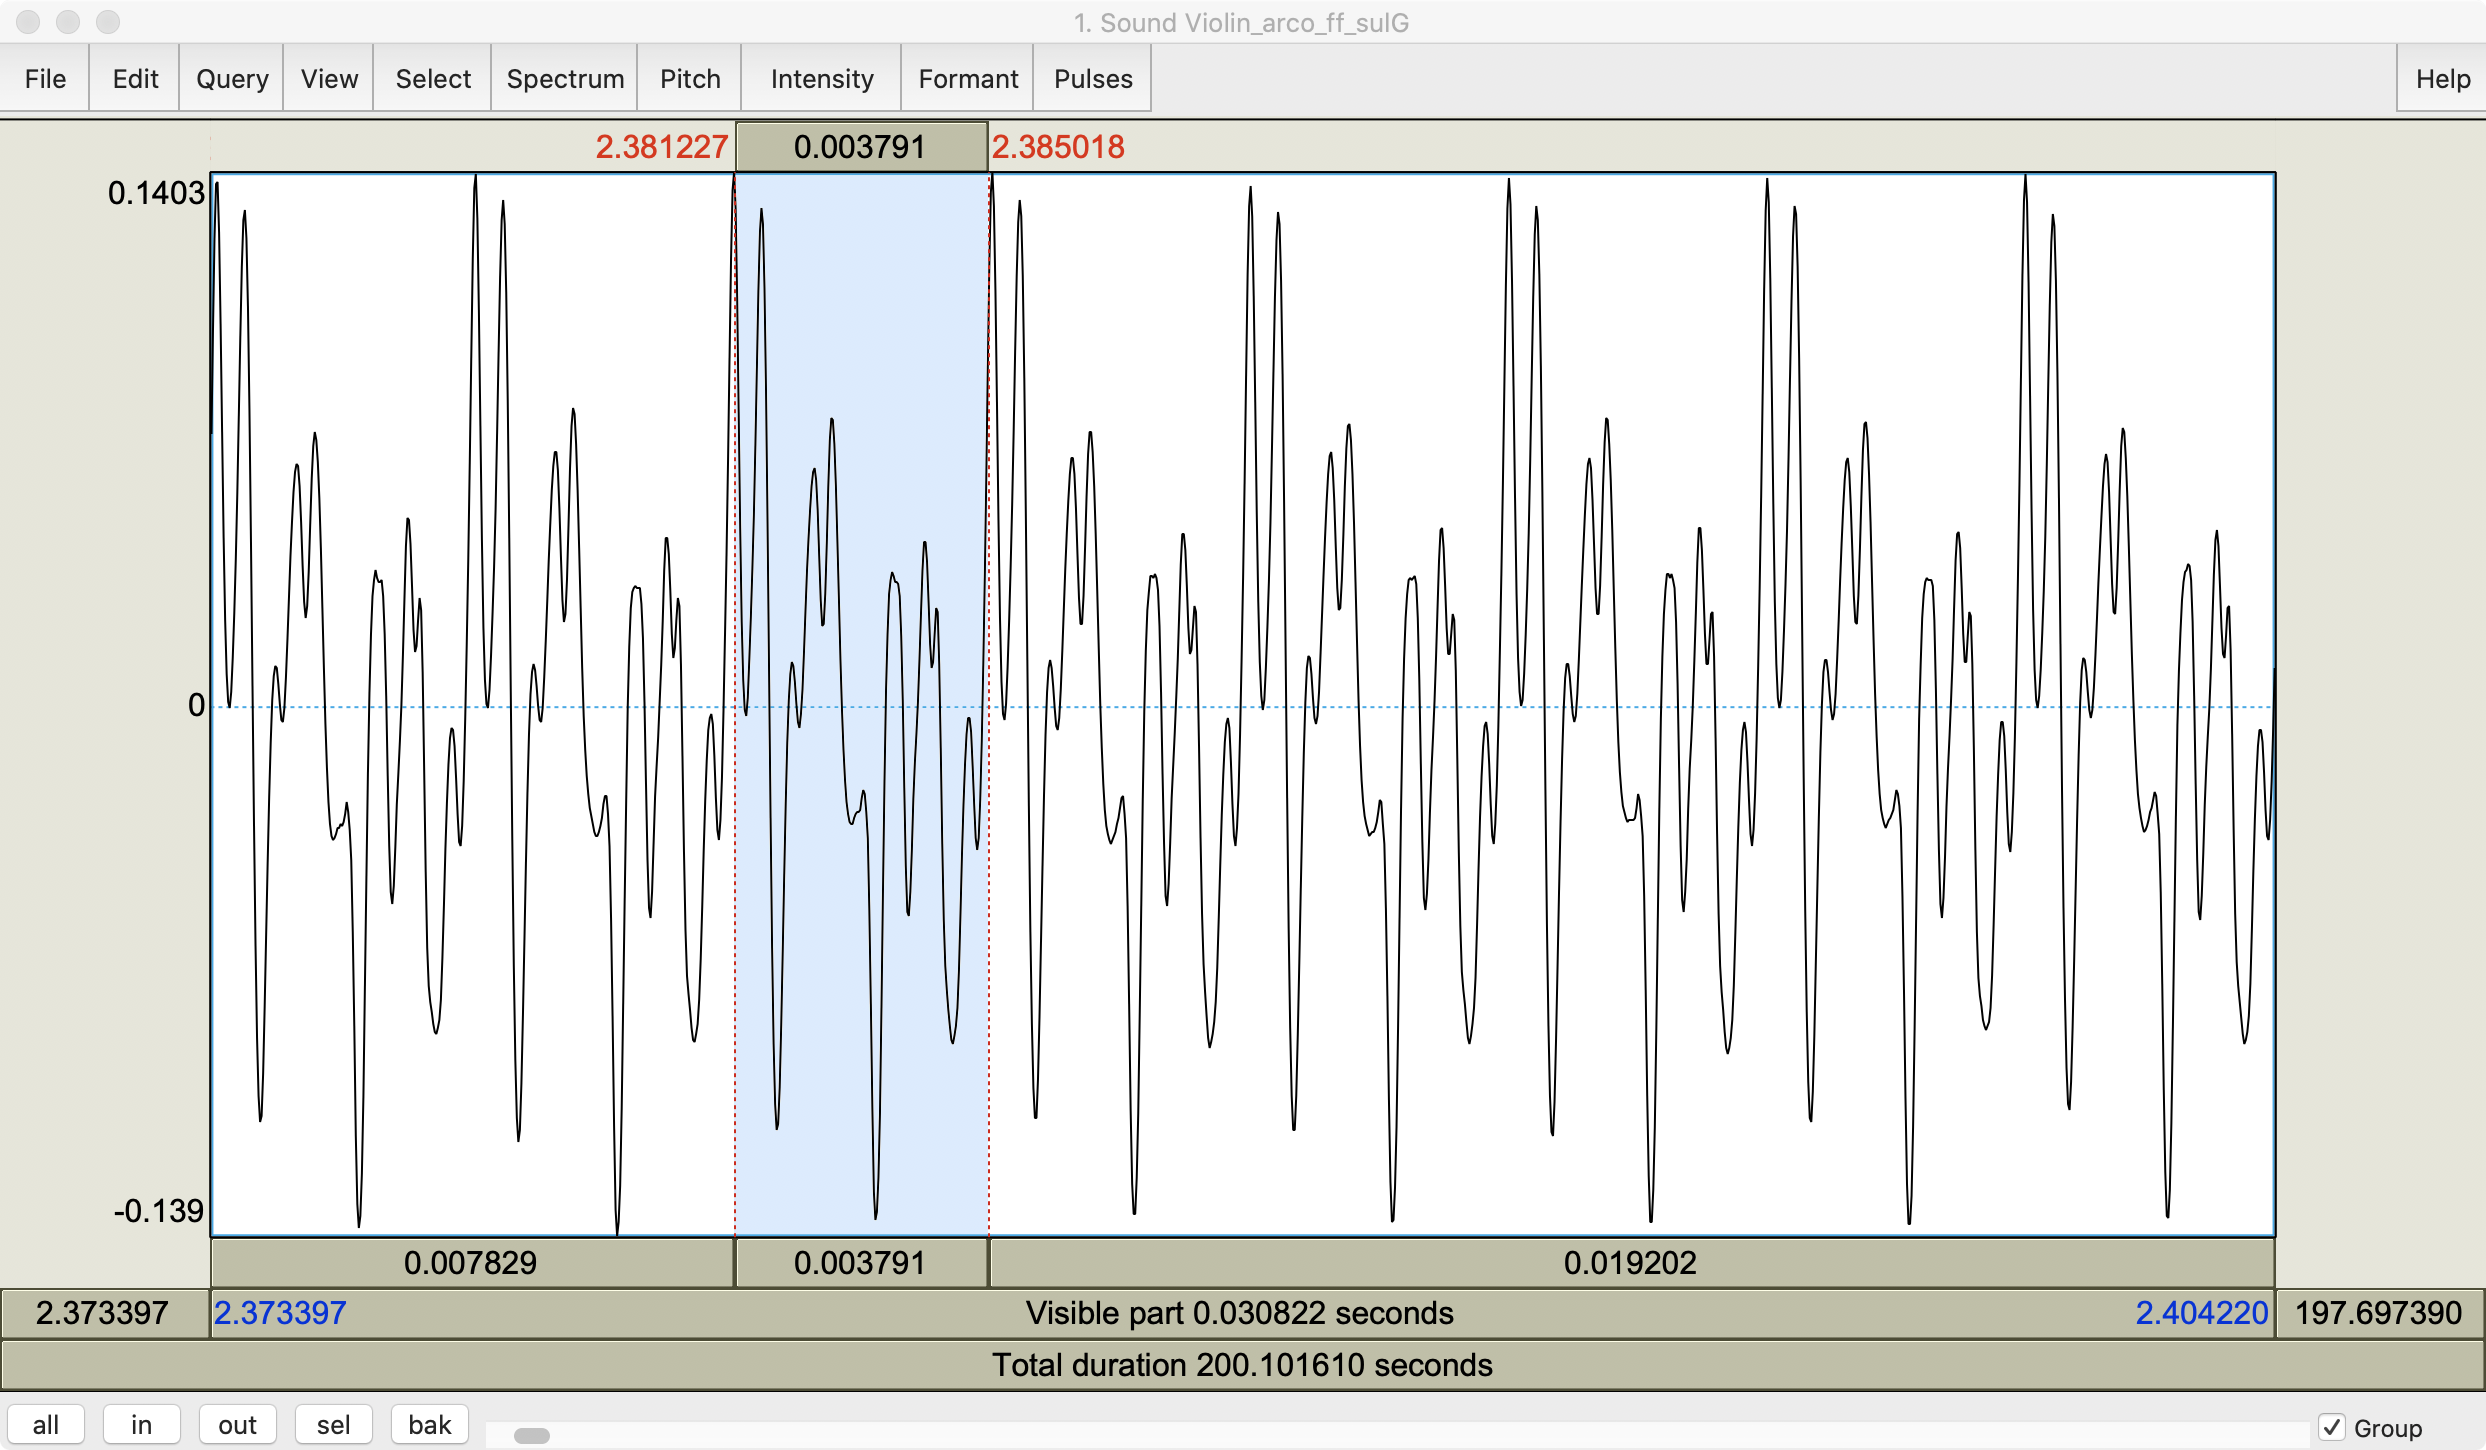
\includegraphics[height=2in]{violin_waveform.png}}
    Eight periods from the recording of a violin playing $f=1/0.003791=262$Hz, i.e., C4 (middle C).
    Waveform distributed by
    \href{http://theremin.music.uiowa.edu/MIS.html}{\bf\color{blue}University of Iowa Electronic Music Studios}.
\end{frame}

\begin{frame}
  \frametitle{Example: Violin}

  \centerline{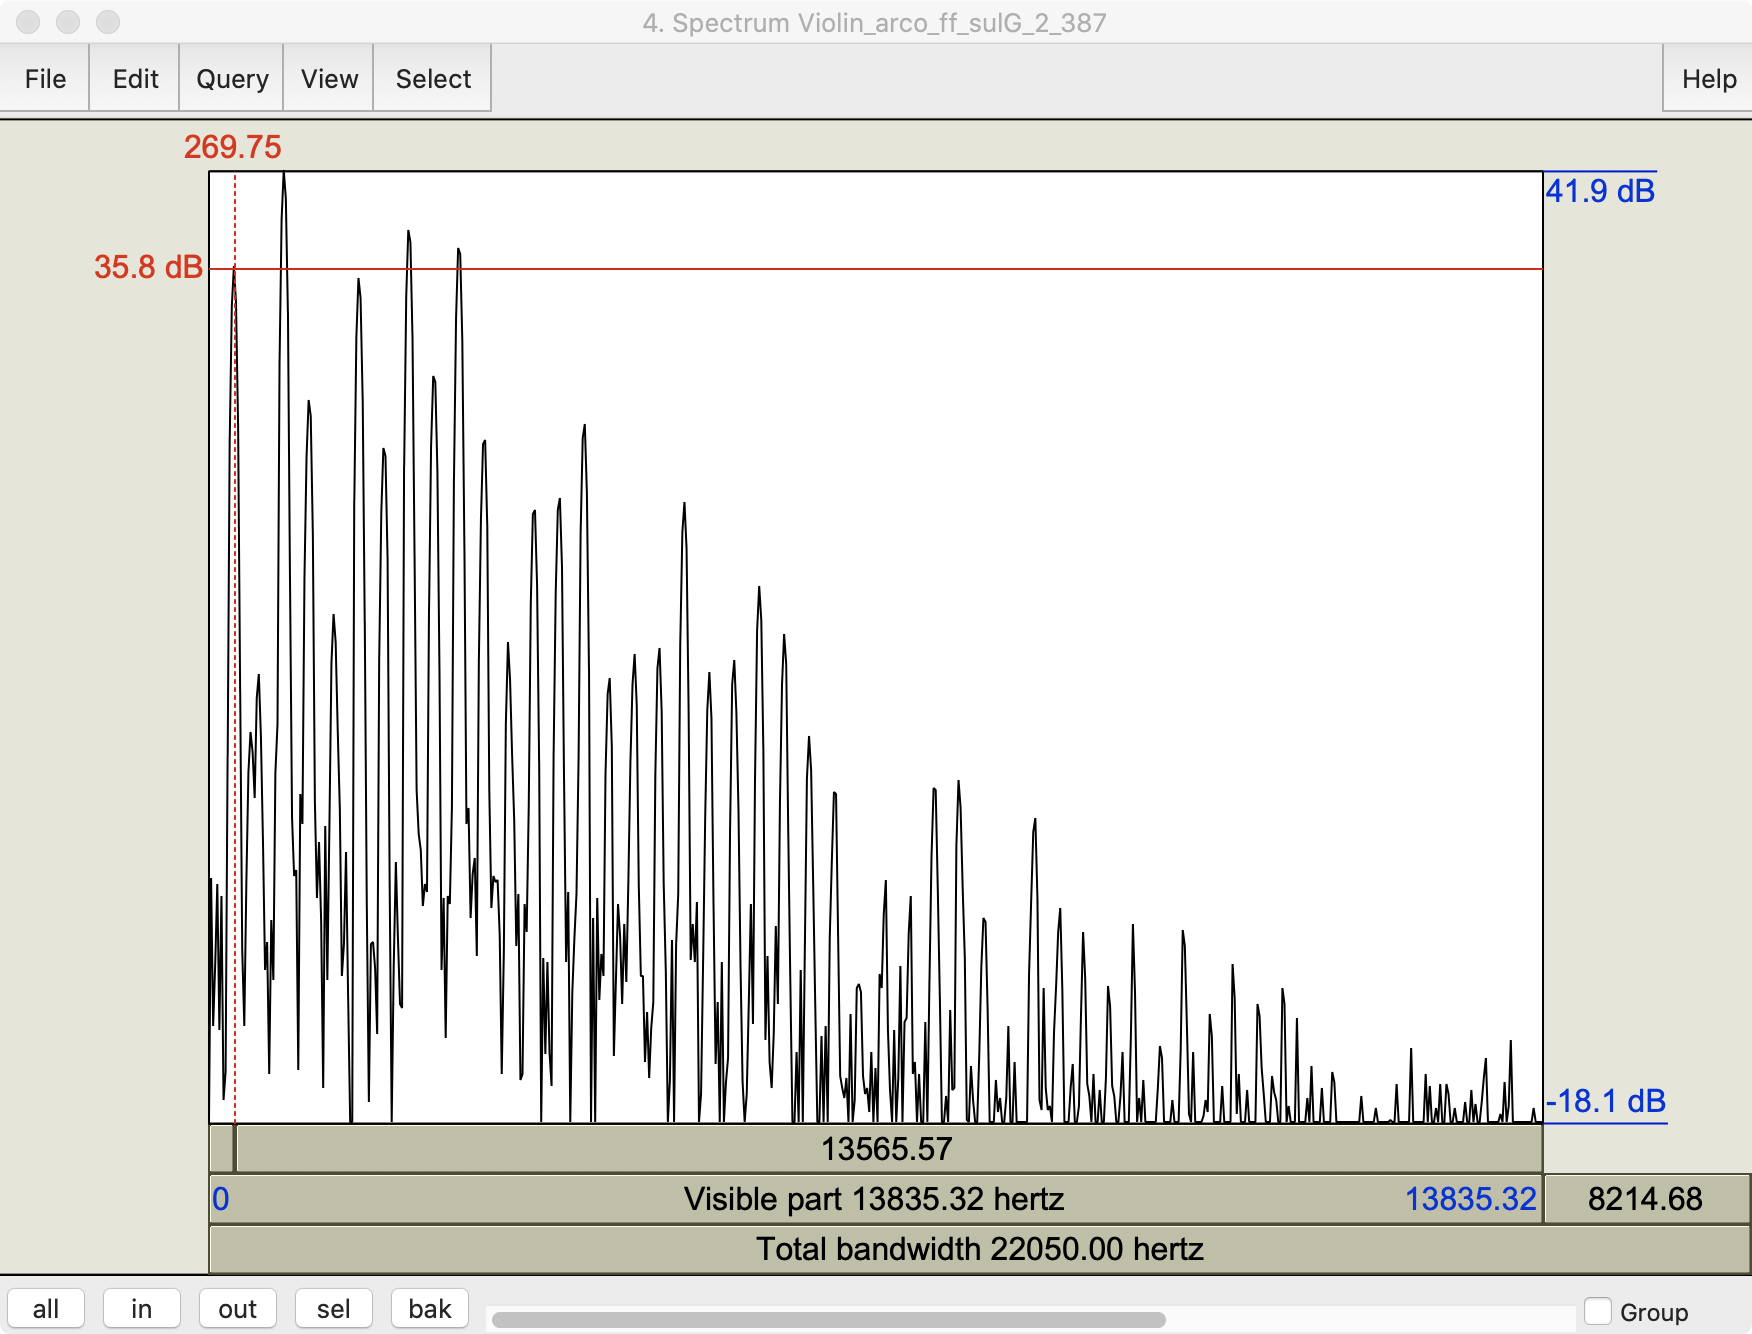
\includegraphics[height=2.5in]{violin_spectrum.png}}
    Log magnitude spectrum ($20\log_{10}|X_k|$) for the first 43 harmonics or so
    ($1\le k\le 43$ or so) of a violin playing C4.
    Waveform distributed by
    \href{http://theremin.music.uiowa.edu/MIS.html}{\bf\color{blue}University of Iowa Electronic Music Studios}.
\end{frame}

%%%%%%%%%%%%%%%%%%%%%%%%%%%%%%%%%%%%%%%%%%%%
\section[Properties]{Properties of a Fourier Spectrum}
\setcounter{subsection}{1}

\begin{frame}
  \frametitle{Properties of a spectrum}

  Spectrum representation is nice to use because
  \begin{itemize}
  \item It's so general.  Any periodic signal can be written this way.
  \item Many signal processing operations can be written directly in
    the spectral domain (as operations on $a_k$), without converting
    back to $x(t)$.
  \end{itemize}
\end{frame}

\begin{frame}
  \frametitle{Property \#1: Scaling}

  Suppose we have a signal
  \[
  x(t) = \sum_{k=-N}^N a_ke^{j2\pi f_kt}
  \]
  Suppose we scale it by a factor of $G$:
  \[
  y(t) = Gx(t)
  \]
  That just means that we scale each of the coefficients by $G$:
  \[
  y(t)  = \sum_{k=-N}^N \left(Ga_k\right) e^{j2\pi f_kt}
  \]
\end{frame}

\begin{frame}
  \frametitle{Property \#2: Adding a constant}

  Suppose we have a signal
  \[
  x(t) = \sum_{k=-N}^N a_ke^{j2\pi f_kt}
  \]
  Suppose we add a constant, $C$:
  \[
  y(t) = x(t) + C
  \]
  That just means that we add that constant to $a_0$:
  \[
  y(t)  = (a_0+C) + \sum_{k\ne 0} a_k e^{j2\pi f_kt}
  \]
\end{frame}

\begin{frame}
  \frametitle{Property \#3: Adding two signals}

  Suppose we have two signals:
  \begin{align*}
    x(t) &= \sum_{n=-N}^N a_n'e^{j2\pi f_n't}\\
    y(t) &= \sum_{m=-M}^M a_m''e^{j2\pi f_m''t}
  \end{align*}
  and we add them together:
  \[
  z(t) = x(t) + y(t) = \sum_k a_ke^{j2\pi f_kt}
  \]
  where, if a frequency $f_k$ comes from both $x(t)$ and $y(t)$, then
  we have to do phasor addition:
  \[
  \mbox{If}~f_k=f_n'=f_m''~~\mbox{then}~~a_k=a_n'+a_m''
  \]
\end{frame}

\begin{frame}
  \frametitle{Property \#4: Time shift}

  Suppose we have a signal
  \[
  x(t) = \sum_{k=-N}^N a_ke^{j2\pi f_kt}
  \]
  and we want to time shift it by $\tau$ seconds:
  \[
  y(t) = x(t-\tau)
  \]
  Time shift corresponds to a {\em\bf phase shift} of each spectral component:
  \[
  y(t) = \sum_{k=-N}^N \left(a_ke^{-j2\pi f_k\tau}\right)e^{j2\pi f_kt}
  \]
\end{frame}

\begin{frame}
  \frametitle{Property \#5: Frequency shift}

  Suppose we have a signal
  \[
  x(t) = \sum_{k=-N}^N a_ke^{j2\pi f_kt}
  \]
  and we want to shift it in frequency by some constant overall shift, $F$:
  \[
  y(t) = \sum_{k=-N}^N a_ke^{j2\pi \left(f_k+F\right)t}
  \]
  Frequency shift corresponds to amplitude modulation (multiplying it by a
  complex exponential at the carrier frequency $F$):
  \[
  y(t) = x(t) e^{j2\pi Ft}
  \]
\end{frame}

\begin{frame}
  \frametitle{Property \#6: Differentiation}

  Suppose we have a signal
  \[
  x(t) = \sum_{k=-N}^N a_ke^{j2\pi f_kt}
  \]
  and we want to differentiate it:
  \[
  y(t) \propto \frac{dx}{dt}
  \]
  Differentiation corresponds to scaling each spectral coefficient by
  $j2\pi f_k$:
  \[
  y(t) = \sum_{k=-N}^N \left(j2\pi f_k a_k\right)e^{j2\pi f_kt}
  \]
\end{frame}

%%%%%%%%%%%%%%%%%%%%%%%%%%%%%%%%%%%%%%%%%%%%
\section[Summary]{Summary}
\setcounter{subsection}{1}

\begin{frame}
  \frametitle{Summary}
  \begin{itemize}
  \item {\bf Spectrum:} The spectrum of any sum of cosines is the set
    of complex-valued spectral coefficients, $a_k$, matched with the
    frequencies $f_k$, such that
    \[
    x(t) = \sum_{k=-N}^N a_ke^{j2\pi f_kt}
    \]
  \item {\bf Fourier's Theorem:} Any periodic waveform,
    $x(t+T_0)=x(t)$, can be synthesized as
    \[
    x(t) = \sum_{k=-\infty}^\infty X_ke^{j2\pi kF_0t}
    \]
  \item {\bf Properties of the spectrum:} signal processing operations
    that can be done directly in the spectrum, without first
    recomputing the waveform, include scaling, adding, time shift,
    frequency shift, and differentiation.
  \end{itemize}
  
\end{frame}

\end{document}
